%
% SECTION
%
\section{Теоретичні основи генетичних алгоритмів}
\subsection{Елементи теорії генетики}
Теорія еволюції Дарвіна передбачає, що еволюція природи --- це процес оптимізації живих організмів. Відповідно до цієї теорії, природний відбір --- це головна умова еволюції в природі.

Суть природного відбору полягає в тому, що більш адаптовані біологічні істоти мають більше шансів на виживання та розмноження. Таким чином, потомки <<кращих>> біологічних індивідів будуть більш пристосовані порівняно зі своїми ровесниками. Отже, через декілька (десятків, сотень, тисяч) поколінь частка адаптованості збільшується в загальній масі~\cite{evolutiontheory}.

%
% SECTION
%
\subsection{Генетичні алгоритми}
\subsubsection{Основні поняття генетичних алгоритмів}
Генетичний алгоритм --- це еволюційний алгоритм пошуку, що використовується для вирішення задач оптимізації і моделювання шляхом послідовного підбору, комбінування і варіації шуканих параметрів з використанням механізмів, що нагадують біологічну еволюцію.

Генетичний алгоритм є комбінацією переборного і градієнтного методів вирішення задач. Механізми схрещування і мутації в якомусь змісті реалізують переборну частину методу, а добір кращих розв’язаннь --- градієнтний спуск~\cite{neural_networks_and_ga}.

Характерними відмінностями генетичного алгоритму є:
\begin{itemize}
	\item обробка не параметрів задачі, а їх закодовану форму;
	\item пошук рішення грунтується не на точці, а на деякій популяції;
	\item при оптимізації використовують тільки цільову функцію;
	\item правила відбору особин популяції імовірнісні.
\end{itemize}

Основні терміни генетичного алгоритму:
\begin{itemize}
	\item особа --- деяке рішення задачі;
	\item хромосома (\textit{chromosome}) --- числовий вектор, що відповідає особі;
	\item ген (\textit{gen}) --- це атомарний елемент хромосоми;
	\item популяція (\textit{population}) --- сукупність особин виду, множина допустимих\\розв’язків;
	\item покоління (\textit{generation}) --- чергова популяція;
	\item функція адаптації (\textit{fitness function}) --- порівняльний показник якості адаптації особи;
	\item  оператор селекції (\textit{selection}) --- це елемент генетичного алгоритму, який відповідає за спосіб вибору осіб, які беруть участь у створенні
наступного покоління;
	\item  оператор схрещування (\textit{crossover}) --- це операція, при якій із двох хромосом породжується одна чи декілька нових хромосом;
	\item  оператор мутації (\textit{mutation}) --- це операція перетворення хромосоми, що випадково змінює одну чи декілька її генів.
\end{itemize}

\subsubsection{Опис алгоритму}
Задача кодується таким чином, щоб її рішення могло бути представлене у виді вектора. Випадковим чином створюється деяка кількість початкових векторів. Вони оцінюються з використанням функції адаптації, у результаті чого кожному векторові привласнюється визначене значення адаптації, що визначає ймовірність виживання організму, представленого даним вектором. Після цього з використанням отриманих значень пристосованості вибираються вектори (селекції), допущені до схрещування. До цих векторів застосовуються генетичні оператори (у більшості випадків схрещування та мутація), створюючи в такий спосіб наступне покоління. Особи наступного покоління також оцінюються, потім виробляється селекція, застосовуються генетичні оператори і т.д. Так моделюється еволюційний процес, що продовжується кілька життєвих циклів (поколінь), поки не буде виконаний критерій зупинки алгоритму. Таким критерієм може бути:
\begin{itemize}
	\item отримання глобального, або субоптимального рішення;
	\item вичерпання числа поколінь, відпущених на еволюцію;
	\item вичерпання часу, відпущеного на еволюцію.
\end{itemize}

Таким чином, можна виділити наступні етапи генетичного алгоритму:
\begin{enumerate}
	\item Створення початкової популяції.
	\item Обчислення функцій адаптації для особей популяції.
	\item[• ] Початок циклу.
	\begin{enumerate}
		\item Селекція.
		\item Схрещування і/або мутація.
		\item Обчислення функцій пристосованості для всіх особей.
		\item Формування нового покоління.
		\item[• ] Якщо виконуються умови зупинки, то алгоритм зупиняється, інакше  перехід до початоку циклу.
	\end{enumerate}
\end{enumerate}

\section{Постановка задачі}
Завданням роботи є знаходження мінімального рішення задачі, яке виражене цільовою функцією на області допустимих рішень, використовуючи генетичні алгоритми та пакет програмного забезпечення MATLAB.

Необхідно провести дослідження створеного алгоритму, а саме оцінити точність результату роботи алгоритму та визначити вплив розміру популяції. 

Згідно з індивідуальним завданням, цільовою функцією є ступенчата функція Де Йонга
\[ f(x) = \sum_{i=1}^{n} [|x_i|],\:x\in(-5.12;5.12),\]
\begin{itemize}
	\item[де] $[|x_i|]$ --- модуль цілої частки $x_i$.
\end{itemize}

%
% SECTION
%
\section{Виконання задачі}
\subsection{Дослідження цільової функції}
Графік ступінчастої функції Де Йонга для двох параметрів представлено на рисунку~\ref{fig:plot_de_jong}.

\begin{figure}[H]
  \centering
    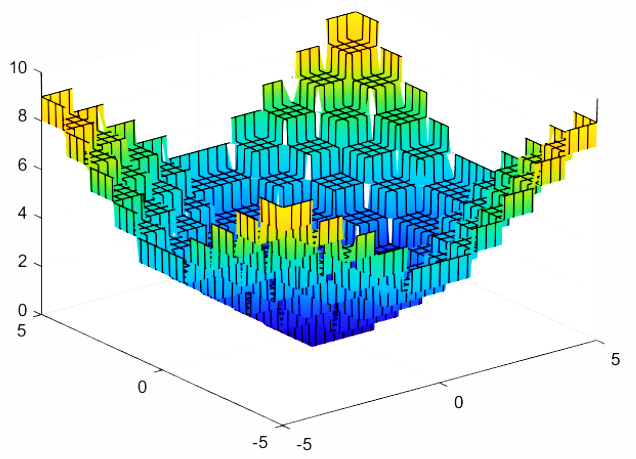
\includegraphics[width=0.6\textwidth]{images/plot_de_jong}
  \caption{Графік функції Де Йонга}
  \label{fig:plot_de_jong}
\end{figure}

Функція має глобальний мінімум в області $x,y\in(-1; 1)$. 

\subsection{Проектування генетичного алгоритму}
Для розрахунку було взято популяцію розміром в 80 осіб, що генерується автоматично у діапазоні згідно з завданням. 

Функція селекції --- стохастична (\textit{selectionstochunif}) --- кожна особа розміщується на колесі рулетки та має розмір секції, пропорційний до її функції адаптації; алгоритм один раз вибирає випадкове число і кожен раз крутить колесо на це число градусів, вибираючи нову популяцію~\cite{site:matlab_ga_options}.

Функція мутації --- мутація по Гаусу (\textit{mutationgaussian}) --- до числа додається випадкове число з розподілу Гаусу~\cite{site:matlab_ga_options}.

Функція схрещування --- рівномірний кросовер (\textit{crossoverscattered}) --- кожний ген має власну імовірність бути успадкуваним від батьків~\cite{site:matlab_ga_options}.

Скрипт для середовища MATLAB: 
\lstinputlisting{code/matlab_ga.m}

\subsection{Аналіз результатів роботи генетичного алгоритму}
Результатом виконання скрипту є 
\[x_1=0.234, x_2=-0.781,\]
\[f(
\begin{bmatrix}
    x_1& x_2
\end{bmatrix}
)=0,\]
отже генетичний алгоритм успішно знайшов глобальний мінімум функції.
Вихідна інформація роботи алгоритму представлена у таблиці~\ref{tab:output}.

\begin{table}[H]
  \centering
    \caption{Процес виконання алгоритму}
    \begin{tabular}{| c | l | l | l | l |}
    \hline
    № & Кількість особин & Найкращий $f(x)$ & Середній $f(x)$ & Застійні покоління \\ \hline
    1 & 160 & 0 & 4.487 & 0 \\ \hline
    2 & 240 & 0 & 2.763 & 1 \\ \hline
    3 & 320 & 0 & 1.9 & 2 \\ \hline
    4 & 400 & 0 & 1.212 & 3 \\ \hline
    5 & 480 & 0 & 0.825 & 4 \\ \hline
    6 & 560 & 0 & 0.6 & 5 \\ \hline
    7 & 640 & 0 & 0.225 & 6 \\ \hline
    8 & 720 & 0 & 0.0875 & 7 \\ \hline
    9 & 800 & 0 & 0.075 & 8 \\ \hline
    10 & 880 & 0 & 0.075 & 9 \\ \hline
    11 & 960 & 0 & 0.075 & 10 \\ \hline
    12 & 1040 & 0 & 0.075 & 11 \\ \hline
    13 & 1120 & 0 & 0 & 12 \\ \hline
    14 & 1200 & 0 & 0 & 13 \\ \hline
    15 & 1280 & 0 & 0 & 14 \\
    \hline
    \end{tabular}
    \label{tab:output}
\end{table}

Функція приймає значення глобального мінімуму на першому поколінні, отже доречним буде зменшити розмір популяції. Процес оптимізації був перерваним через досягнення заданої кількості поколінь. Графік динаміки функції адаптації представлено на рисунку~\ref{fig:plot_dynamic}.

\begin{figure}[H]
  \centering
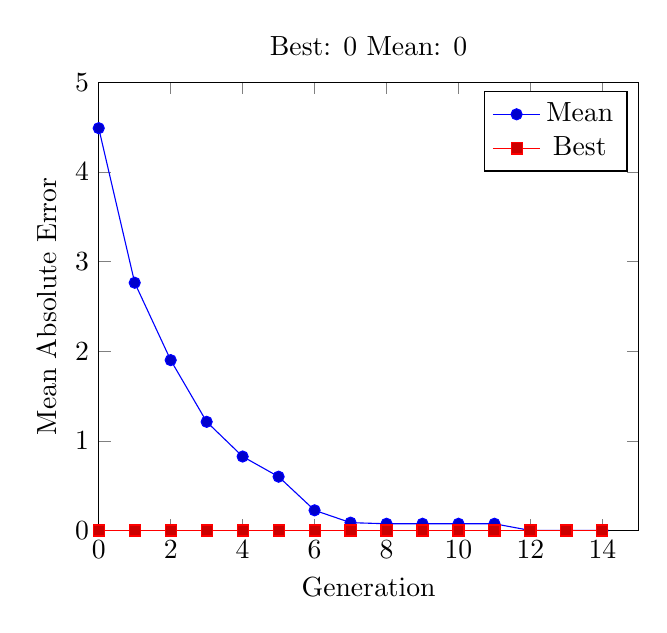
\begin{tikzpicture}
  \begin{axis}[ 
    title={Best: $0$ Mean: 0},
    xlabel={Generation},
    ylabel={Mean Absolute Error},
    xmin=0,xmax=15,ymin=0,ymax=5
  ] 
	\addplot
		coordinates {
			(0,4.487) [0]
			(1,2.763) [1]
			(2,1.9) [2]
			(3,1.212) [3]
			(4,0.825) [4]
			(5,0.6) [5]
			(6,0.225) [6]
			(7,0.0875) [7]
			(8,0.075) [8]
			(9,0.075) [9]
			(10,0.075) [10]
			(11, 0.075) [11]
			(12,0) [12]
			(13,0) [13]
			(14,0) [14]
		};
	\addlegendentry{Mean}
	\addplot
		coordinates {
			(0,0) [0]
			(1,0) [1]
			(2,0) [2]
			(3,0) [3]
			(4,0) [4]
			(5,0) [5]
			(6,0) [6]
			(7,0) [7]
			(8,0) [8]
			(9,0) [9]
			(10,0) [10]
			(11,0) [11]
			(12,0) [12]
			(13,0) [13]
			(14,0) [14]
		};
	\addlegendentry{Best}
  \end{axis}
\end{tikzpicture}
  \captionsetup{justification=centering}
  \caption{Графік динаміки функції адаптації (розмір популяції 80)}
  \label{fig:plot_dynamic}
\end{figure}

Для перевірки припущення про змешення розміру популяції, розмір було змінено з 80 до 5. При таких умовах глобальний мінімум був досягнутий на 2 генерації (рисунок~\ref{fig:plot_dynamic_2}). 

\begin{figure}[H]
  \centering
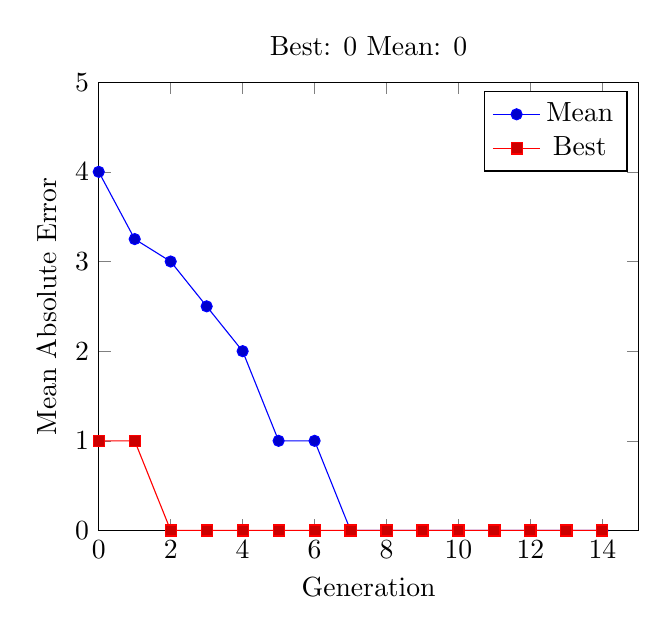
\begin{tikzpicture}
  \begin{axis}[ 
    title={Best: $0$ Mean: 0},
    xlabel={Generation},
    ylabel={Mean Absolute Error},
    xmin=0,xmax=15,ymin=0,ymax=5
  ] 
	\addplot
		coordinates {
			(0,4) [0]
			(1,3.25) [1]
			(2,3) [2]
			(3,2.5) [3]
			(4,2) [4]
			(5,1) [5]
			(6,1) [6]
			(7,0) [7]
			(8,0) [8]
			(9,0) [9]
			(10,0) [10]
			(11, 0) [11]
			(12,0) [12]
			(13,0) [13]
			(14,0) [14]
		};
	\addlegendentry{Mean}
	\addplot
		coordinates {
			(0,1) [0]
			(1,1) [1]
			(2,0) [2]
			(3,0) [3]
			(4,0) [4]
			(5,0) [5]
			(6,0) [6]
			(7,0) [7]
			(8,0) [8]
			(9,0) [9]
			(10,0) [10]
			(11,0) [11]
			(12,0) [12]
			(13,0) [13]
			(14,0) [14]
		};
	\addlegendentry{Best}
  \end{axis}
\end{tikzpicture}
  \captionsetup{justification=centering}
  \caption{Графік динаміки функції адаптації (розмір популяції 5)}
  \label{fig:plot_dynamic_2}
\end{figure}

%
% SECTION
%
\section*{Висновки} 
\addcontentsline{toc}{section}{Висновки}
За допомогою генетичних алгоритмів у пакеті MATLAB була вирішена задача знаходження мінімуму функції і досліджено вплив  розміру популяції на точність обчислень. З використанням пакету MATLAB можна швидко дослідити роботу генетичного алгоритму, побудувати графік динаміки фітнес-функції. 
